\chapter{Framework for Symbiotic Development}\label{cha:chapter2}}

The concept of peer-to-peer applications is not new, nor is the concept of distributed hash tables. 
What emerged in 2008 with the publication of the Bitcoin white paper was an incentive structure that unified these two software paradigms with a set of economic stimuli to motivate the creation of a dedicated computing network orders of magnitude more powerful than the world's fastest supercomputers.
The purpose of which is the maintenance of a massive distributed database known as the Bitcoin blockchain.
Apart from the digital currency it enables, blockchain technology is a fascinating new computing paradigm with broad implications for the future development of the World Wide Web, and by extension, the further growth of Linked Data and the Semantic Web. This chapter is divided into two main sections, we first demonstrate how blockchain technologies can contribute towards the realization of a more robust Semantic Web, and subsequently we provide a framework wherein the Semantic Web is utilized to ameliorate blockchain technology itself.

\section{Background}

With the rise of the Bitcoin cryptocurrency the concept of distributed blockchain databases received wider attention.
Based on the distributed blockchain infrastructure a wide range of distributed applications can be built.
One unique approach in that regard is Etherum platform, which includes a Turing-complete programming framework aiming to realize so called ``\textit{smart contracts}''.
Similarly as blockchain technology can facilitate distributed currency, trust and contracts application, Linked Data facilitated distributed data management without central authorities.
In this article, we investigate how the blockchain and Linked Data concepts can be fruitfully combined to realize novel applications.
%Cryptographic hash tables in the form of Merkle trees, viz. blockchain, as popularized by the open-source Bitcoin project have been garnering significant attention in popular culture and media but to date have not been thoroughly examined in the context of the utility of its application to semantic technologies. 
%change this first sentence

One of the problems with the blockchain as a technology is the negative association it has inherited due to the illicit nature of some early applications of Bitcoin as a currency. Moreover the polarization of it's advocates, who often regard it as a panacea, i.e. ``\textit{the most important invention in the history of the world}''\footnote{\footnotesize{http://rogerver.com}}, and vehemence or apathy of its detractors, e.g. Jamie Dimon the chief executive officer of JPMorgan Chase, quick to write it off completely as a ``\textit{waste of time}''\footnote{\footnotesize{http://fortune.com/2015/11/04/jamie-dimon-virtual-currency-bitcoin}}, has contributed towards an environment wherein it is difficult to isolate the novel contributions of blockchain technology, of which there are some, and how they might be harnessed to improve the infrastructure of the Web, a development we regard as both desirable and actionable. 

This chapter proceeds with a two-pronged demonstration, first we provide an objective analysis of blockchain technology in the context of its relevance to the Semantic Web.
% In so doing we hit upon legacy issues in the design of the Web, and by implication the Linked Data infrastructure, that blockchain computing stands to resolve. 
With our framework firmly established we go on to describe a methodology for the implementation of several applications made possible through the integration of well known Semantic Web concepts within the computational architecture of the blockchain and set forth a benchmark for evaluating the validity of our approach.

In the subsequent sections we provide a high level description of the functional underpinnings of the Bitcoin blockchain and examine two technologies that extend the current blockchain in ways applicable to the contribution we describe above. 
Furthermore we demonstrate our model of a blockchain based URI naming scheme that positions the RDF data model in closer alignment with the concept of Cool URIs~\cite{timbernerslee1998}. 
Next is a description of the composition of an extensible ontology for blockchains and the resultant Linked Data ecosystem in the context of exploring the exchange of value within a network as well as the unification of the disparate technical nomenclature, towards creating a common understanding of analogous components existing in silos of the development landscape this open-source community continues to foster.
Finally we examine the case for novel semantic applications of decentralized Industry 4.0 platforms. 


\section{Context}

The blockchain facilitates a resilient and highly distributed ledger for recording transactions, attributing them to a specific node in a network, and ordering them in time. 
This is the functionality that undergirds the cryptocurrency Bitcoin (BTC), among others. This phenomenon is made possible through a process known as ``\textit{mining}'' whereby a large number of dedicated high-powered computers running application-specific integrated circuits (ASICs)~\cite{grantbrunner2013} process the transactions of the Bitcoin network in real time, competing with each other for a small fee associated with a new transfer in BTC in addition to a ``\textit{subsidy}'' in the form of a fixed amount of newly minted Bitcoins.
Data is permanently recorded in the Bitcoin network through files called blocks. 
A block is a record of some or all of the most recent Bitcoin transactions that have yet to be recorded in prior blocks. 
Mining is the process of adding transaction records to Bitcoin's public ledger of past transactions. 
This ledger of past transactions is called the blockchain as it is a chain of blocks. 
The blockchain serves to confirm transactions to the rest of the network as having been executed.

\subsubsection{Blockchain}

A useful analogy for conceptualizing blockchain technology is peer-to-peer (P2P) computing, wherein a distributed application architecture partitions work loads among equally privileged participants in an application, forming a peer-to-peer network of nodes.
A blockchain is a globally shared, transactional database, similar to the peer-to-peer file sharing system BitTorrent. 
All participants in a blockchain network can read the database. 
Where it diverges from P2P applications is in the ``\textit{consensus}'' mechanism. 
Changes in the database are performed by means of transactions, which have to be accepted by the participants in the network. 
Transactions are atomic (i.e. executed in full), durable (i.e. can not be altered) and cryptographically signed by the creator (guarding access to modifications of the database). 
\autoref{fig:block-chain-risk} illustrates the blockchain concept. 
Several transactions are bundled in a block and then executed and distributed among the nodes in the blockchain network. 
In case of conflicting transactions, the first one is given precedence and subsequent conflicting ones are discarded.

\begin{figure}[tb]
   \center 
   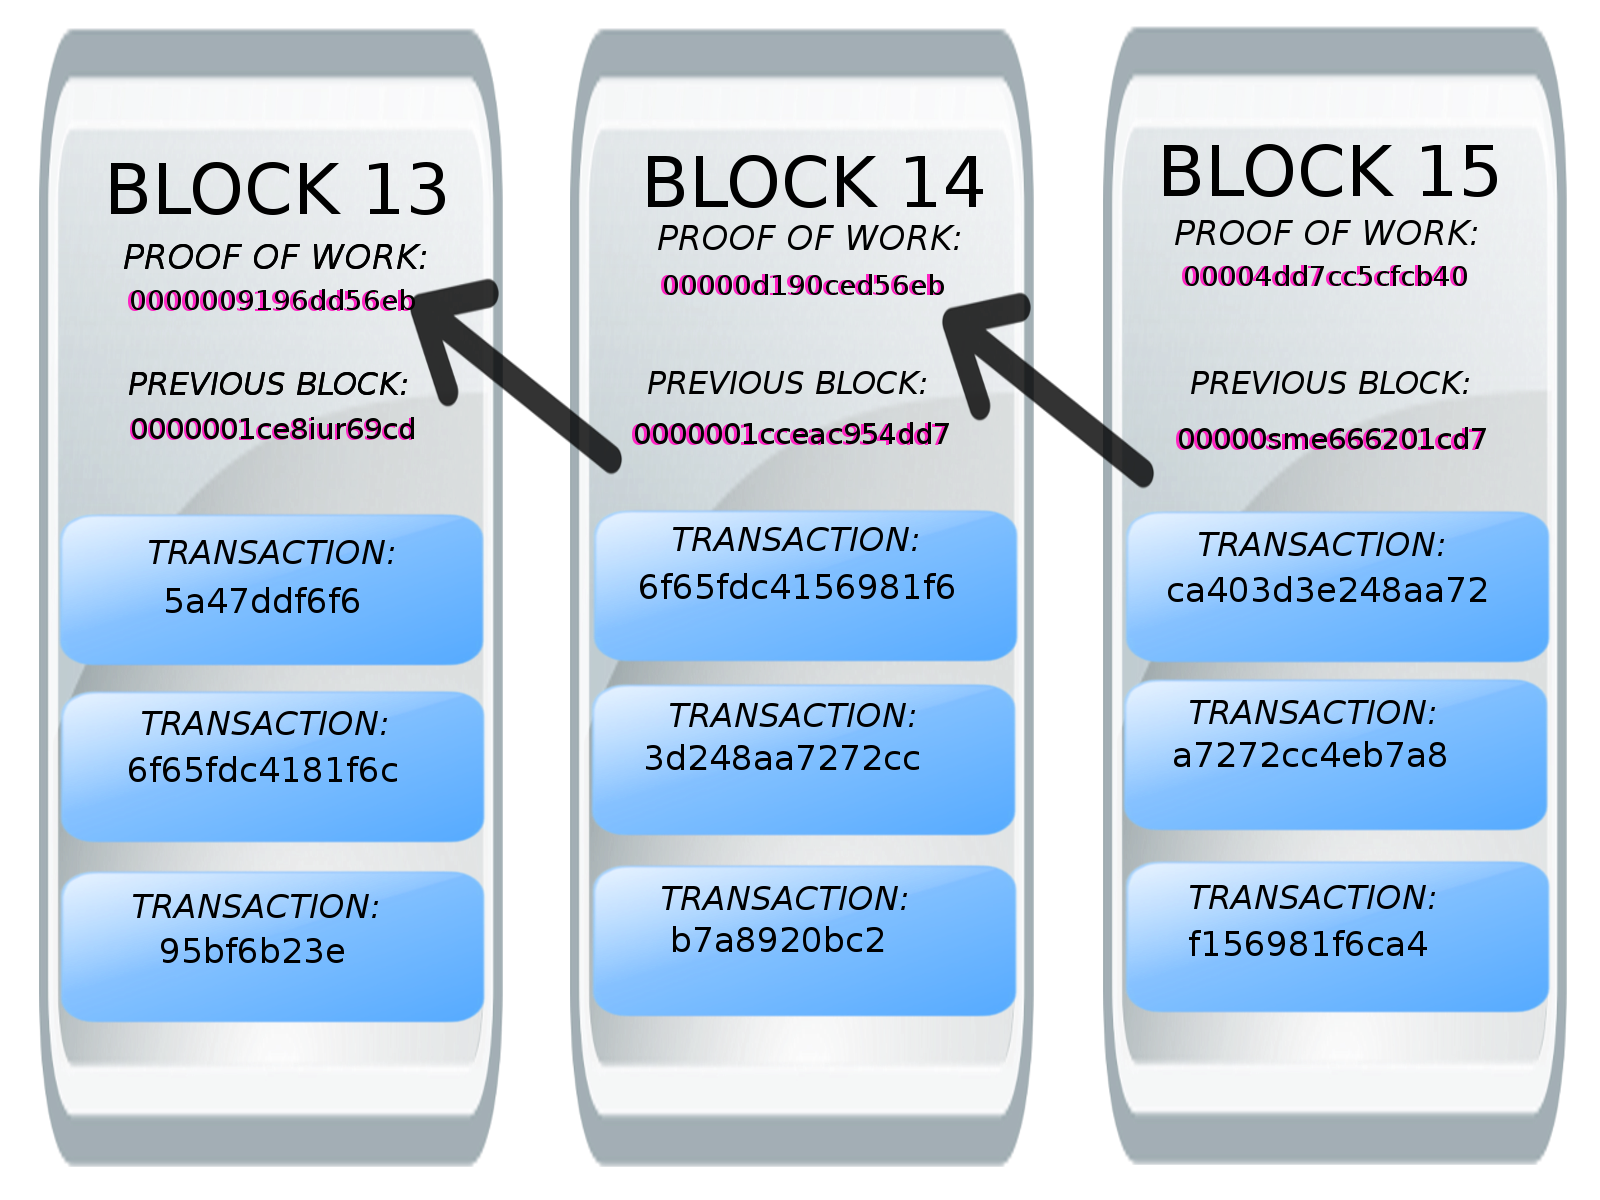
\includegraphics[width=.7\textwidth]{blockchain_sme}
   \caption{Illustration of a Blockchain} 
   \label{fig:block-chain-risk}
\end{figure} 
 

\subsubsection{Blockchain 2.0.}

The securing of a cryptocurrency network notwithstanding, there are a multitude of applications that can be run alongside, or in conjunction with the Bitcoin blockchain, taking advantage of the large amount of computational effort generated by the dedicated mining machines and the open access afforded to this processing power available to all holders of even nominal amounts, i.e. 0.00000001 (known as 1 \textit{Satoshi} after the author of the original white paper~\cite{whitepaper}), of BTC. 

Furthermore there are numerous forks of the original open-source Bitcoin code, known as ``\textit{altcoins}'', the majority of which implement negligible or generally uninteresting modifications. That said, in this paper we explore two of such forks that have extended the original blockchain concept in ways which can be utilized to provide useful and unique services, extending the blockchain concept in powerful ways. 

Bitcoin's scripting language allows one to store small amounts of metadata on the blockchain, which can be used to represent transactions more complex than simple exchange such as asset manipulation instructions, i.e. escrow services that cannot release a transaction without consent from multiple parties. 
These ancillary applications have come to be known collectively as ``\textit{Blockchain 2.0}''.

\subsubsection{``Smart Contracts''}

The original blockchain network can be regarded as a tool to execute a system of contracts focused on the application of value exchange. Altcoins such as Namecoin adapted this original ``\textit{currency application}'' of the technology into other applications, in the case of Namecoin, to DNS registration. 
Ethereum is another Altcoin project which attempts to build a more generalised blockchain technology; on which all transaction-based state machine concepts can be built, to provide to the end-developer a tightly integrated end-to-end system for building software on a hitherto unexplored compute paradigm in the mainstream: a trustful object messaging compute framework, i.e. performing non-trivial computations within the blockchain itself~\cite{wood2014ethereum}.
While the Bitcoin blockchain does allow very simple transactions (i.e. the transfer of funds from one account to another), Ethereum expands the concept of transactions to arbitrary complex contracts dubbed ``\textit{smart contracts}''. For this purpose, transactions contain an algorithmic description of the smart contract and Ethereum provides programming languages and APIs for devising the smart contract. 

\subsubsection{Ethereum Virtual Machine}

The Ethereum Virtual Machine (EVM) is the runtime environment for smart contracts in Ethereum.  It is sandboxed and completely isolated (i.e. code running inside the EVM has no access to network, filesystem or other processes). Smart contracts even have limited access to other smart contracts. 
In subsequent sections we explore how the extended functionality of ``\textit{smart contracts}'' could potentially facilitate a series of novel methods for the symbiotic development of blockchain technologies with the Semantic Web. 


\section{What can blockchain do for Semantic Web?}

In the preceding sections we examined the novel computational paradigm that blockchain as a technology makes feasible. In this section we will demonstrate ways in which blockchain technology can be applied in practice towards the actualization of a more resilient architecture for the Semantic Web. 

\subsection{Secure Resource Identifiers}

On the Semantic Web, all information is expressed in statements about resources.
Resources are identified by International or Uniform Resource Identifiers (IRI/URIs). 
While URIs are very beneficial, they also have some inherent weaknesses:

\begin{itemize}
    \item \emph{Centralization.} While individual URIs can be minted in a distributed fashion, the identifier generation relies on the centralized DNS system, which poses a single point of failure or attack.
    \item \emph{Persistence.} In case of intentional (e.g. a merger or acquisition of a legal entity) or unintentional (e.g. bankruptcy) events, the persistence of identifiers can not be guaranteed.
\end{itemize}

There are three key requirements which an ideal identifier system should fulfill:

\begin{enumerate}
    \item \emph{Secure:} dereferencing identifiers should not be prone to attacks, i.e. when retrieving the content of a website or resource the authenticity of the content should be ensured.
    \item \emph{Human-readable:} it should be possible to give identifiers intuitive names, which can be easily remembered by humans.
    \item \emph{Decentralized:} no central authority should control identifier creation and pose a single point of failure or attack.
\end{enumerate}

Zooko Wilcox-O'Hearn conjectured that no single kind of naming system can achieve more than two of these properties~\cite{wilcox2003names}.
Aaron Swartz~\cite{aaronswartz2011} described a naming system based on Bitcoin employing Bitcoin's distributed blockchain as a proof-of-work to establish consensus of domain name ownership.
These systems remain vulnerable to an attack wherein the reputation system is subverted by forging identities in the peer-to-peer network but is secure under Byzantine fault tolerance.

Namecoin implements the concept.
Namecoin is a decentralized open source information registration and transfer system based on the Bitcoin blockchain itself.
It enables users to dis-intermediate the Domain Name System (DNS) providers, one of the last bastions of centralization in the architecture of the modern web.

Practically speaking the issues identified above have afflicted the Semantic Web community in the past, e.g. the shuttering of Freebase by it's acquirer Google~\cite{2015}. 
Consider the semantic machine learning system NELL (Never-Ending Language Learning)~\cite{carlson2010toward}, which aims at remaining operational indefinitely. 
For such an ambition as this to be credible we must rely on a system that satisfies the aforementioned criteria, a system such as Namecoin. 
Consequently we have commenced the implementation of a fully functional mirror site to \texttt{dbpedia.org} under the top-level domain \texttt{dbpedia.bit}.
To achieve success in this endeavour there are some technical hurdles to overcome, we detail these now.  

On the protocol level, there are no constraints on URIs in Namecoin; names can be made up of arbitrary binary data with a length of 0 to 255 bytes. If we want a \texttt{.bit} DNS name, in Namecoin syntax the name should be structured as ``\texttt{d/example}'' where ``\texttt{example}'' must be a lower-case, valid domain name. 
New resources are assigned subdomains to \texttt{dbpedia.bit}. 
\autoref{fig:sparql} demonstrates a simple exemplary query on the de-referenceable blockchain based naming scheme for DBpedia under the domain `\texttt{dbpedia.bit}'.

\begin{lstlisting}[label=fig:sparql,caption=SPARQL query on \texttt{.bit} TLD,language=Javascript,basicstyle=\scriptsize \ttfamily,numbers=left,numberstyle=\tiny\color{mygray}]
PREFIX ex: <http://dbpedia.bit/exampleOntology#>
SELECT ?capital ?country WHERE {
  ?x ex:cityname      ?capital ;
     ex:isCapitalOf   ?y .
  ?y ex:countryname   ?country ;
     ex:isInContinent ex:Europe .
}
\end{lstlisting}


In terms of long-term viability, names on this system can be transferred and thus also sold. 
It is even possible to sell names in a trust-less way in exchange for Namecoin currency, since the transaction sending the name and the transaction paying the seller can be made atomic.
If a wallet owning a name disappears the name expires 36,000 blocks after the last update, so it will stay active for some time but then become available again for a new owner.

\subsection{Namecoin Access}

The Namecoin blockchain stores the pertinent information for navigating the \texttt{.bit} top level namespace. However, since \texttt{.bit} domain names, are not yet part of the standard domain name system, these can not be de-referenced without additional support. For example, there are \texttt{.bit} web proxy servers that will correctly handle these DNS requests in a browser as well as extensions for Firefox, Chrome and online look up services\footnote{\footnotesize{\texttt{http://namecha.in/name/d/domob}}}.
To dereference or retrieve resources from \texttt{dbpedia.bit} run the core client, using the ``\texttt{name\_show}'' RPC command,  e.g. ``\texttt{name\_show d/domob}'' on the debug console, or ``\texttt{namecoin-cli name\_show d/domob}'' on the shell.

\subsection{Storing data in the blockchain}

There are multiple ways to store data directly within the Bitcoin blockchain. 

\begin{enumerate}
 \item \emph{Value:} Encode data in the number of \textit{Satoshis} being sent to an address.
 \item \emph{Vanity address:} Brute force through keys until arriving at an address that encodes personalized data, i.e. encoding the pattern \texttt{1ESWC} as in \\ \texttt{1ESWCs3d48d3198863e75m7f9d1827cdfc6048e}.
 \item \emph{MultisigAddress:} These are more complex Bitcoin addresses that require more than one signature from a private/public key to redeem the value.
 \item \emph{OP\_RETURN:} Command in the Bitcoin scripting language that was specifically added to permit the inclusion of metadata (up to 40 bytes) on the blockchain.
\end{enumerate}

Moreover, units of real world value distinct from the blockchain can be affixed to nominal amounts of BTC, as stock certificates were once printed on paper, the paper itself has some small value, but it represents (presumably) a greater value insofar as it is the physical manifestation of part ownership in some corporation. A so-called ``\textit{colored coin}'' is used in conjunction with a wallet specially tailored to recognize such additional information, thereby conferring the benefits of the blockchain's distributed trust mechanism to a multiplicity of novel applications~\cite{timswanson2014}. We regard this as the most feasible medium of synthesis between blockchain and representations of information in the Linked Data ecosystem.  

\section{What can Semantic Web do for blockchain?}

Through formal semantic knowledge representations we have created an ontology for capturing data within the blockchain.
The utility of such a shared conceptualization is twofold.
Primarily it facilitates a shared understanding of blockchain concepts between humans.
Additionally, by exposing the blockchain data according to an ontology, we enable interlinking with other Linked Data to conduct formal reasoning and inference. 

Our work extends, in keeping with the principles of ontology reuse~\cite{grangel2015Convention}, an initial vocabulary created by Melvin Carvalho~\cite{melvincarvalho2013}\footnote{\url{http://cc.rww.io/vocab}}. In so doing we formalize key concepts such as wallets, blocks and transactions.
We render the vocabulary suitable for graphical analysis using Visual Notation for OWL Ontologies~\cite{VOWL2}.
%cite irlan

\begin{figure}[tb]
   \center 
   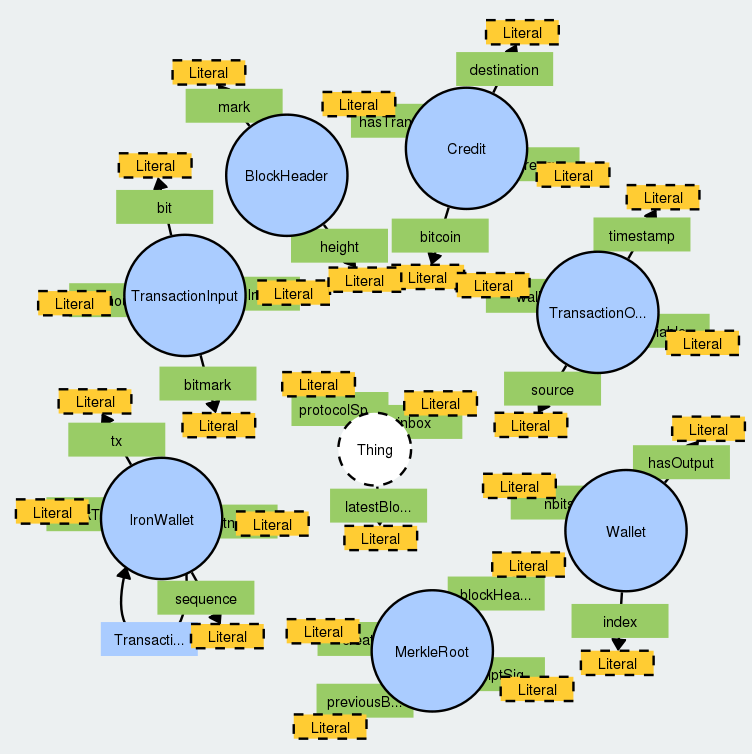
\includegraphics[width=.5\textwidth]{vocab_visualization_0}
   \caption{Diagram Illustrating the Ontology} 
   \label{fig:viz}
\end{figure} 


\subsection{Exploring the blockchain}

One of the beneficent features of blockchain technology is that it increases transparency through a completely open ledger (in order to establish trust) while simultaneously ensuring anonymity through preserving accounts behind their public keys.
However, the transparency is currently only established on a technical level.
For humans it is cumbersome to track transactions and accounts on the blockchain.
The vocabulary based representation of the blockchain data increases transparency and analysis capabilities for human users.
We propose a model whereby transactions are represented in RDF, and thereby support the linking of wallets related by transactions to follow exchange activity around the network.
The first generation of blockchain explorers\footnote{\url{http://blockchain.info/}} are limited in efficacy by the aforementioned issue, as in \autoref{fig:api} transactions represented in JSON are notoriously difficult to follow throughout the network.

\begin{lstlisting}[label=fig:api,caption=JSON Exploration API Output,language=Javascript,basicstyle=\scriptsize \ttfamily,numbers=left,numberstyle=\tiny\color{mygray}]
{
    "balance" : 43.50100000,
    "errors" : "",
    "paytxfee" : 0.005,
    "proxy" : "",
    "connected" : 0,
    "testnet" : false,
    "difficulty" : 1733207.51384839,
    "blocks" : 179602
}
\end{lstlisting}

Our working ontology, implemented in OWL, melds the Carvalho vocabulary with the Bitcoin API calls list \footnote{\url{http://en.bitcoin.it/wiki/Original_Bitcoin_client/API_calls_list}}.
Furthermore we include functionality to actualize the working model of Ethereum smart contracts. 
However, since Ethereum is in an early stage of development, further changes are likely to be required in the future.
Additions comprise in particular the ability to bind the validity of transactions to certain geospatial locations, to facilitate the generation of so-called ``\textit{smart property}'', property whose ownership is controlled via the blockchain, with access contingent upon ownership of a public/private key pair~\cite{szabo1997idea}.


\subsection{Testnet Block Explorer}

The term ``\textit{testnet}'' is used to refer to a blockchain created by forking the original Bitcoin code repository\footnote{\footnotesize{\texttt{http://github.com/bitcoin}}}, configuring several nodes, and commencing the mining process on one's own machine or local network. 
This practice is the primary mechanism for blockchain-based experimentation. 
Naturally testnet coins are distinct from Bitcoins ``\textit{in the wild}'', they are not intended to denote monetary value, permitting iterative development without large capital outlays or adverse effects to the main Bitcoin blockchain.

Transactions can be described using our working blockchain vocabulary\footnote{\footnotesize{\texttt{http://github.com/smenglish/block.chain.ontology}}}. 
The supplementary information thereby created can be injected into the blockchain by one of several methods: 

\begin{itemize}
    \item The coinbase field of a mined block allows for hexadecimal data which can hold 560 bytes.
    
    \item Use of a ``\textit{colored coin}'' and corresponding specialized wallet.
    
    \item Multiple outputs can be used for a transaction such that each holds hexadecimal data. This would imply dust value outputs (outputs of $\leqslant{}$ 0.00005640 BTC) and in practice would contribute relatively ``\textit{large}'' amounts of superfluous data to the blockchain, a technique known as ``\textit{bloating}'' and generally considered bad practice.
    
    \item Hexadecimal data from a multi-signature transaction can also be used to encode information.
\end{itemize}

The open-source \textit{Block Explorer}\footnote{\footnotesize{\url{http://testnet.blockexplorer.com}}} can be used to examine the contents of transaction blocks, i.e. recipient and sender addresses or code snippets delivered through counterparty exchanges and recorded in the testnet blockchain as depicted in \autoref{fig:testnet}.  


\begin{lstlisting}[label=fig:testnet,caption=Testnet Output Specifying Counterparties,language=Javascript,basicstyle=\scriptsize \ttfamily,numbers=left,numberstyle=\tiny\color{mygray}]
{
  "sender": "1QBb5MpKUMiqc27wrD2QDRsC9gZYyy49",
  "recipient": "1AdCDBz2VmhUZDyDbibMo2QGGSjt93zbF",
  "size": 479,
  "merkleroot": "f5b3309272c5fcb3febb0f09986e77158",
  "time": 1440604813,
  "bits": "1814434",
  "difficulty": 54256630327.88996,
  "reward": 25,
}
\end{lstlisting}


\begin{figure}[tb]
   \center 
   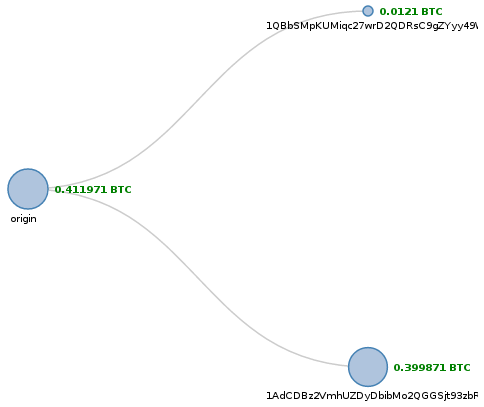
\includegraphics[scale=0.3]{Alfa_beta_tree}
   \caption{Graphical Representation of Linked Transaction Counterparties} 
   \label{fig:block-chain-explorer}
\end{figure} 


Describing transactions in the context of Linked Data, as contrasted with a less expressive representation, facilitates a number of benefits. Binding transactions to individuals or organizations in furtherance of transparency, or to a particular geographic location as in the execution of so called ``\textit{smart property}'' arrangements. 
In \autoref{fig:block-chain-explorer} we demonstrate how such a transaction propagates through our network, with many of such applications taking place there is an emergent linked data ecosystem of value transmission.

\subsection{Standardization}

At the time of writing, contributors to the core Bitcoin blockchain code number less than four hundred individuals\footnote{\footnotesize{\texttt{http://github.com/bitcoin/bitcoin/graphs/contributors}}}.
If blockchain technology will become an integral component in the infrastructure of the modern Web it will necessitate its being thoroughly understood by a much greater community of developers. 
The lack of such a common understanding was cited as one of the premiere issues impeding this continued growth of blockchain technology by Gavin Andreeson the successor to Satoshi Nakamoto as the principal maintainer of the bitcoin code base~\cite{jonmatonis2012}.
Accordingly we have contributed to a the creation of the first publicly-available\footnote{\footnotesize{\texttt{http://github.com/smenglish/block.chain.ontology}}} shared ontology to facilitate improved comprehension within this burgeoning development community.

\subsubsection{Industry 4.0}

The fourth industrial revolution, Industry 4.0, is a collective term embracing a number of contemporary automation, data exchange and manufacturing technologies. It had been defined as ``a collective term for technologies and concepts of value chain organization''~\cite{nirjargandhi2015} which draws together Cyber-Physical Systems, the Internet of Things and the Internet of Services, and critically Semantic Technologies. In this section we consider the ways the union of blockchain technologies and the Semantic Web is shaping the continued development of this latest phase of industrialization. 

\begin{figure}[tb]
   \center 
   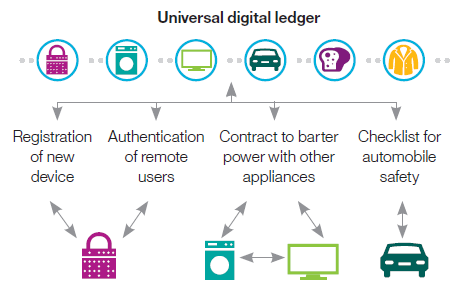
\includegraphics[width=.7\textwidth]{i40ledger}
   \caption{Using the blockchain as universal digital ledger for Industry 4.0 transactions~\cite{DeviceDemocracy}.} 
   \label{fig:passport}
\end{figure} 

Using blockchain technology, a fully decentralized data marketplace for sensor data could be realized. Instead of establishing individual contracts with every data provider, the blockchain could become a clearing house for sensor data exchange. In \cite{DeviceDemocracy} IBM describes the vision of employing the blockchain as universal digital  ledger for Industry 4.0  transactions, such as registration of devices, authentication of users, bartering and supply chain transparency. For these applications, a comprehensive semantic description of the products and half-products exchanges in the value chain is essential. Finally, such descriptions should be linked with related information contained in other systems of the participating companies.

As a concrete example, \autoref{fig:provenance} shows the core logic of a Ethereum ``\textit{smart contract}'', which represents an address on an Industry 4.0~\cite{christopherbrewster2014} supply chain management platform.
The \texttt{mortal} super-class defines the initialization and finalization of the smart contract.
The contract \texttt{accountManager} itself comprises a potentially large array indexed by accounts with each entry comprising two pieces of information, an URI identifying a certain product type and possibly linking to further information about the product as well as a hash identifying a concrete product realization or production batch.
The public key authentication of Ethereum ensures only a certified account owner can update information about the provenance of his products or semi-products.
If other participants in the supply chain, refer to such a product or semi-product (e.g. in a way that it is incorporated/used within their product) the public ledger based on the Etherum blockchain ensures, the provenance of products and their incorporated half-products and ingredients can be traced back along the supply chain.

\begin{lstlisting}[label=fig:provenance,caption=Simple Ethereum Contract on Industry 4.0 Platform \texttt{Provenance.org}~\cite{juttasteinerjessibakergavinwood2013},language=Javascript,basicstyle=\scriptsize \ttfamily,numbers=left,numberstyle=\tiny\color{mygray}]
contract mortal {
    /* Define variable owner of the type address*/
    address owner;
    /* this function is executed at initialization and sets the owner of the contract */
    function mortal() owner = msg.sender;
    /* Function to recover the funds on the contract */
    function kill() if (msg.sender == owner) suicide(owner);
}
contract accountManager is mortal {
    /* data structure to hold accounts*/
    struct Account {
        string uri;
        bytes32 hash;
    }
    /* mapping of accounts to data*/
    mapping (address => Account) accounts;
    function setAccount(string uri, bytes32 hash) returns (bool)
        return setAccount(msg.sender, uri, hash);
    function setAccount(address account, string uri, bytes32 hash) returns (bool) {
        bool rv = msg.sender == owner || msg.sender == account;
        if (rv) accounts[account] = Account(uri, hash);
        return rv;
    }
    function readAccountUri(address account) constant returns (string)
        return accounts[account].uri;
    function readAccountHash(address account) constant returns (bytes32)
        return accounts[account].hash;
}
\end{lstlisting}


\section{Discussion}

In this chapter we have endeavoured to catalogue the results of a thorough analysis of blockchain technology in terms of it's applicability as a computational paradigm to the Semantic Web and Linked Data community. Furthermore we have presented the results of our initial efforts to fuse these two constructs in mutually beneficial ways by extending the traditional Linked Data naming convention, providing an ontology for representation of elements and events in the blockchain ecosystem, and building a procedure for Link Data representation of transactions in a blockchain network. We have done a first step towards synergisticly integrating two promising decentralized data management technologies, Linked Data and blockchains.
It is the first step on a larger research agenda aiming to realize a truly distributed, democratic and domain-agnostic knowledge system.

% At present we are undertaking efforts to apply our approach more generally to the Bitcoin blockchain itself, we are interested in a comprehensive graphic analysis in RDF of the entire Bitcoin blockchain, specifically one that is generalizable to \textit{altcoins} as well. The dynamic nature of the Ethereum implementation codebase made it difficult to implement and test some of the ideas described in this article. We plan to create a comprehensive implementation and evaluation of integrating the Linked Data concepts into the Ethereum blockchain.